% Figure 2: one round trip on nazuna (QEMU/KVM, one pinned vCPU), p50, ns.
% Data: research-plan.md M8, M12, M14, M16, M17. Linux is NATIVE on the host,
% not in the VM (owed: Linux in the same VM).
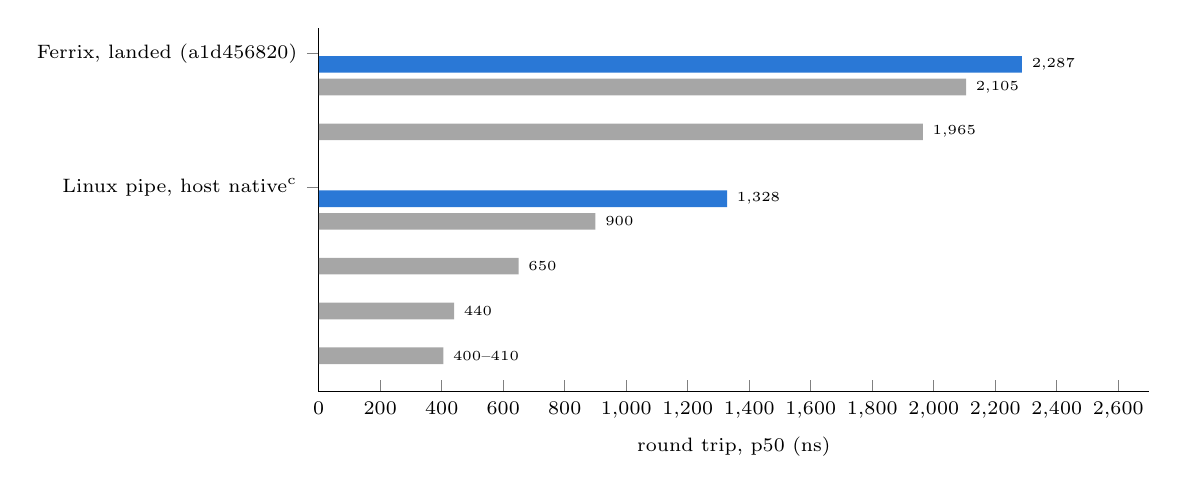
\begin{tikzpicture}
\begin{axis}[
  width=\columnwidth, height=6.2cm,
  xbar, bar width=6pt, xmin=0, xmax=2700,
  xlabel={round trip, p50 (ns)},
  ytick=data, y dir=reverse,
  yticklabels={
    {Ferrix, landed (a1d456820)},
    {Linux pipe, host native\textsuperscript{c}},
    {Redox 0.9.0, scheme},
    {Ferrix, step 4 (unlanded)\textsuperscript{b}},
    {seL4, \texttt{IBPB} each switch},
    {seL4, defaults},
    {seL4, matched},
    {seL4, matched, no refill}},
  yticklabel style={font=\scriptsize},
  xticklabel style={font=\scriptsize}, xlabel style={font=\scriptsize},
  nodes near coords, nodes near coords style={font=\tiny, anchor=west},
  point meta=explicit symbolic,
  axis x line*=bottom, axis y line*=left,
  enlarge y limits=0.08,
]
\addplot[fill={rgb,255:red,42;green,120;blue,214}, draw=none] coordinates {
  (2287,0) [2,287] (1328,3) [1,328] };
\addplot[fill=black!35, draw=none] coordinates {
  (2105,1) [2,105] (1965,2) [1,965] (900,4) [900] (650,5) [650] (440,6) [440] (405,7) [400--410] };
\end{axis}
\end{tikzpicture}
